\section{Bayesian Approach Results}\label{s:results}
We test the ability of PES-P to solve optimization problems in three cases with
increasing realism from the optimization of randomly generated objective
functions drawn from a GP, to the tuning of feedback gains of random linear
systems and a neuromuscular walking model. In all cases, we compare the
performance of the proposed algorithm to the expected improvement criterion (EI)
(\cref{eq:expected_improvement}) and random sampling via Latin hypercubes
(LH)\sidenote[][2.25in]{LH sampling divides the parameter space into ${(2N)}^D$
hypercubes, where $D$ is the dimensionality of the space. $2N$ samples are
placed such that each hypercube has at most one sample and there is at most one
filled hypercube along any row of hypercubes when viewed along any direction.
This method ensures that the samples are roughly uniformly distributed in the
entire space. At each iteration we choose two of these
samples.}~\citep{mckay2000comparison}. For the three simulated cases, we show
results over 20 trials and measure performance in terms of the immediate regret,
defined as $IR = |f(\tilde x_n^*) - f(x^*)|$, versus the number iterations.
Here, $f(\tilde x_n^*)$ is the objective value of the current estimate of the
optimum at this iteration, $f(x^*)$ is the value of the true optimum, and an
iteration consists of a single preference query between two points.
Additionally, we also check the statistical significance of the reduction in IR
obtained by PES-P compared to both EI and LH via two-sided Mann-Whitney $U$
tests $(p < 0.05)$.

\begin{figure*}[t!]
    \centering
    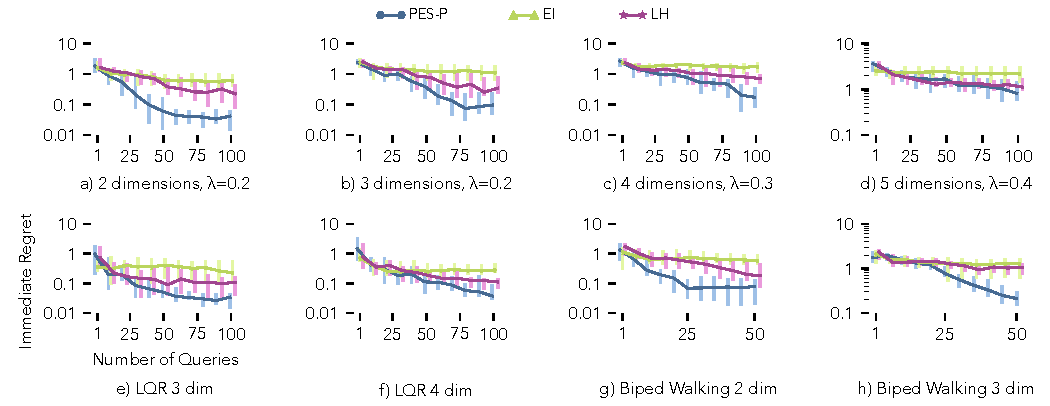
\includegraphics[width=\textwidth]{pes_results}
    \caption[Comparison of Preference-based Bayesian optimization
    methods]{Performance of predictive entropy search with preferences (PES-P),
    expected improvement (EI), and Latin hypercube random sampling (LH) for
    optimizing random objective functions sampled from a GP (a-d), and tuning
    feedback control parameters of random linear systems (e-f) and a biped
    walking model (g-h). Shown are the median and interquartile range over 20
    trials of the immediate regret (IR) against the number of preference
    queries. Black stars indicate iterations for which PES-P achieves
    statistically significant stochastic reductions in IR compared to both EI
    and LH according to two-sided Mann-Whitney $U$ tests $(p <
    0.05)$.}\label{fig:y_err_sim}
\end{figure*}

\subsection{Optimizing Randomly Generated Objective Functions}

To avoid inducing bias by hand-engineering test functions, we first evaluate the
algorithm on random synthetic objective functions. We generate objective
functions on the domain $x \in {[-1, 1]}^D$ by sampling a vector of 500 function
values from a GP prior with a quadratic mean, $\mu(x) = - x^\tn{T} x$, and
isometric squared exponential covariance $\funcil{k}{x_i,x_j} = \exp
\left(\frac{-1}{2 \lambda} x_i^T x_j \right)$. We use a quadratic mean function
to bias the function distribution away from those that have their optimum on a
boundary of the domain, as these functions are easier to optimize. We continue
to generate the rest of the function as it is optimized by conditioning the GP
on the 500 seed values and all function values sampled during the optimization.
We assume the mean of the final function distribution is the true objective
function. To simulate more realistic situations, we provide the algorithms with
noisy preferences from the sampled function values ($\sigma^2 = 0.1$).

Figures~\ref{fig:y_err_sim}a-d show the immediate regret for two to five
dimensional problems with $\lambda$, the length scale of the kernel, scaling
from 0.1 to 0.4 as the dimensionality of the problem increases. On two to four
dimensional problems, PES-P outperforms EI and LH by achieving statistically
significant reductions in IR\@. However, as the dimensionality increases, it
takes more iterations for this advantage to become apparent. In the five
dimensional case, there is no significant difference between PES-P and LH,
likely due to $M=12$ samples of $x_m^*$ being insufficient and the difficulty of
accurately sampling $x_m^*$ in higher dimensions.

\subsection{Tuning Controllers for Random Linear Systems}
Next, we test the ability of PES-P to optimize simple control systems by
optimizing the feedback gains $K$ for $D$-dimensional single-input linear
systems $\dot{\xi} = A \xi + Bu$ with feedback $u = K \xi$. We sample the
elements of the $A$ matrix from the standard normal distribution while $B =
{[0_{1 \times (D-1)}, 1]}^\tn{T}$. We assume a quadratic instantaneous cost
resulting in the objective function
\begin{equation}
    f(K) = - \int_0^{t_f} \xi_K^\tn{T}(t) (Q + K^T R K) \xi_K(t) dt,
\end{equation}
where $\xi_K(t)$ is the evolution of the state under the control policy $K$ and
a fixed initial condition $\xi_0$, $Q = I_{D \times D}$ and $R = 1$. To obtain a
finite search domain, we find the stable range of parameters by varying the
elements of the true optimal control parameters $K^*$ one at a time while
keeping other elements constant. We scale and shift this region to map to the
domain ${[-1, 1]}^D$. Finally, we use the Automatic Relevance Determination
Gaussian Kernel and optimize the hyperparameters at each iteration by maximizing
the posterior probability of the hyperparameters under a gamma
hyperprior~\citep{chu2005preference,
williams2006gaussian}. In order to apply a consistent noisy preference model
$(\sigma^2 = 0.1)$ across all sampled systems, we transform all objective values
by first mapping them through $-\log(-f(K))$ and then shifting and scaling the
values by the mean and range of the values of $10^D$ randomly sampled
controllers. 

Figures~\ref{fig:y_err_sim}e and~\ref{fig:y_err_sim}f show the resulting
optimization performance on three and four dimensional systems. In the 3
dimensional case, PES-P achieves a lower median IR than LH after 30 iterations.
This difference becomes significant after 60 iterations. In the 4 dimensional
case, PES-P significantly outperforms LH after 50 iterations, but the
significance of this improvement is sporadic as the iterations continue. A
possible reason for the reduced performance difference between PES-P and LH in
the LQR problem as compared to the random objective function problems is the
existence of hard-to-optimize flat regions in the LQR objective functions. This
suggests that PES-P may be more well suited for problems that have clear
optimum.
\subsection{Tuning Control Parameters of a Walking Model
    }\label{sec:sim_neuro}
In the third case, we test the ability of PES-P to optimize the feedback gains
for a neuromuscular model of walking~\citep{thatte2016toward}, a system with a
complex non-linear controller addressing the specific application domain of
human locomotion. We perform two and three dimensional optimizations, in which
we tune the feedback gains for a subset of the model's muscle actuators.  We use
the negative cost of transport plus the distance walked over a 20 second time
span as the objective function. As in the previous linear systems example, we
obtain noisy preferences between parameters and optimize the hyperparameters at
every iteration.

Figures~\ref{fig:y_err_sim}g and~\ref{fig:y_err_sim}h show the performance of
PES-P, EI, and LH\@. In this example, PES-P achieves a significant reduction in
IR in just 10 iterations in the 2-dimensional case and in 25 iterations in the 3
dimensional case.  Furthermore, in the 3D case the PES-P's median solution is
approximately 10 times better than those found by EI or LH\@. 
